% 2961w - 30p

\documentclass[12pt,letterpaper]{article}
\usepackage{natbib}
\usepackage{pdflscape}
\usepackage{fullpage}
\usepackage{url}
\usepackage{epsfig}
\usepackage{caption}
\usepackage{hyperref}
\usepackage{enumerate}
\usepackage{dcolumn}
\usepackage{lineno}
\usepackage[T1]{fontenc}
\usepackage{textcomp}
\usepackage{float}
\usepackage[osf]{mathpazo}
\restylefloat{table}
\newcolumntype{d}[1]{D{.}{.}{#1}}

\pagenumbering{arabic}


%Pagination style and stuff
\linespread{2}
\raggedright
\setlength{\parindent}{0.5in}
\setcounter{secnumdepth}{0} 
\renewcommand{\section}[1]{%
\bigskip
\begin{center}
\begin{Large}
\normalfont\scshape #1
\medskip
\end{Large}
\end{center}}
\renewcommand{\subsection}[1]{%
\bigskip
\begin{center}
\begin{large}
\normalfont\itshape #1
\end{large}
\end{center}}
\renewcommand{\subsubsection}[1]{%
\vspace{2ex}
\noindent
\textit{#1.}---}
\renewcommand{\tableofcontents}{}
%\bibpunct{(}{)}{;}{a}{}{,}

%---------------------------------------------
%
%       START
%
%---------------------------------------------

\newcommand{\treats}{\texttt{treats} }

\begin{document}

%Running head
\begin{flushright}
Version dated: \today
\end{flushright}
\bigskip
\noindent RH: \treats package.

\bigskip
\medskip
\begin{center}

\noindent{\Large \bf \treats: a modular \texttt{R} package for simulating trees and traits.} 
\bigskip

\noindent {\normalsize \sc Thomas Guillerme$^{1,*}$}\\
% , Natalie Cooper$^{2}$, Andrew P. Beckerman$^{1}$, and Gavin H. Thomas$^{1,3}$
\noindent {\small \it 
$^1$School of Biosciences, University of Sheffield, Sheffield, S10 2TN, United Kingdom.\\
% $^2$Natural History Museum, Cromwell Road, London, SW7 5BD, United Kingdom.\\
% $^3$Bird Group, Department of Life Sciences, the Natural History Museum at Tring, Tring, United Kingdom.\\
}

\end{center}
\medskip
\noindent{*\bf Corresponding author.} \textit{guillert@tcd.ie}\\  
\vspace{1in}

%Line numbering
\modulolinenumbers[1]
\linenumbers

%---------------------------------------------
%
%       ABSTRACT
%
%---------------------------------------------


% 3000-4000 words


\newpage
\begin{abstract} 

    \begin{enumerate}
        \item Simulating biological realistic data can be an important step to understand and investigate biological mechanisms.
        Simulated data can be used to generate null, base line or neutral models.
        These models can be used either in comparison to observed data to estimate the mechanisms that generated the data.
        Or they can be used to explore, understand and develop theoretical advances by proposing toy models.

        \item In evolutionary biology, such simulations often involve the need of an evolutionary process where descent with modification is at the core of how the simulated data is generated.
        These evolutionary processes can then be nearly infinitely modified to include much more complex processes to affect the simulations such as traits co-evolution, competition mechanisms or mass extinction events.

        \item Here I present the \treats package, a modular \texttt{R} package for trees and traits simulations.
        This package is based on a simple birth death algorithm from which all core steps can easily be modified by users (hence the modularity).
        It also provides a tidy interface through the \treats object, allowing users to easily run reproducible simulations.

        \item Here I present the core algorithms and their integrated modularity and provide an example of how to use the \treats package when studying disparity, the diversity of traits.
        The \treats package also comes with an extend manual regularly updated following users' questions or suggestions which comes as an extended supplementary material to this paper.

    \end{enumerate}

\end{abstract}

\noindent (Keywords: trees, traits, simulations, birth-death, null-models, ecology, evolution, disparity)\\

\vspace{1.5in}

\newpage 

%---------------------------------------------
%
%       INTRODUCTION
%
%---------------------------------------------

\section{Introduction}

% Simulations in biology
Comparing biological patterns is one of the key ways to understand mechanisms in evolutionary biology.
This lead to the development of phylogenetic comparative methods as key methodologically driven topic in ecology, evolution and palaeontology \citep{felsensteinPCM,pennell2013review}.
As indicated in the name, phylogenetic comparative methods rely on comparing patterns in a phylogenetic context (i.e. descent with modification) to understand biological mechanisms or concepts \citep{harmon2019book}.
These comparisons can be done between observed patterns under different conditions or against null, neutral or baseline models (see \citealt{bausman2018neutral} for distinctions or common misconceptions) suggesting different processes or mechanisms.
For example different traits distribution for species with different diets \citep{deepak2023diet},
% different habitats https://onlinelibrary.wiley.com/doi/full/10.1111/jbi.12939
or by comparing some observed pattern to one simulated under null or base conditions\citep{miller2022alternating}.
In theory, workers can follow the research pipeline of thinking of a specific mechanism (e.g. mass extinction allowing the surviving species to acquire new morphologies), collect some data to test this mechanism (e.g. some traits of species across and extinction event) and then compare these patterns to one simulated under no specific conditions (e.g. a null model where the traits evolve randomly regardless of an extinction event)\citep{puttick2020complex}.
For such an approach, we need statistical and softwares solutions to simulate trees and data to generate these specific null models.

% What already exists
In practice, these evolutionary simulations can be done relatively easily multiple times on computers using a birth-death process \cite{feller1939birthdeath,stadler2010birthdeath,diversitree}
A birth-death process is @yadiyada and has been routinely implemented in \texttt{R} (\citealt{R}; e.g. \citealt{ape}, \citealt{diversitree}).
Traits can be simulating using the following processes @OU, @BM, @yadidada. % TODO
The diversity of these traits through time can be called disparity in palaeontology \cite{guillerme2020disparities} or functional diversity in ecology (for functional traits; \citealt{mammola2021concepts}).
In \texttt{R}, this can be done with several already well used and well documented packages.
For example if you want to simulate diversity through time, you can use \texttt{TreeSim} \citep{treesim} to simulate diversity under a set of specific parameters (e.g. speciation and extinction) with some events disrupting the simulations (e.g. mass extinctions).
One can even improve on generating these patterns using \texttt{FossilSim} \citep{fossilsim} to generate a pattern that will take into account fossilization processes.
Or use \texttt{paleobuddy} \citep{paleobuddy} or \texttt{paleotree} \citep{paleotree} to generate palaeontology specific data.
On the other hand, if you need to simulate both diversity and traits through time, this can be done with specific parameters in \texttt{RPANDA} \citep{rpanda} or in \texttt{PETER} \citep{puttick2020complex} where the traits are generated stochasticaly through time (given some process) during the birth-death process.



% STOPPED HERE



% The problems with the absence of modularity
Although the packages mentioned above (and more that we forgot to mention/don't know off) and are excellent (i.e. fast, reliable and documented) at the specific tasks they are designed for, they unfortunately don't allow much modifications beyond the parameters implemented for each specific function.
This can be problematic for generating specific simulations to be used as a specific null model for some specific questions.
For example, \texttt{TreeSim} can simulate a birth-death tree with some extinction event but is not designed to simulated one with an extinction event that leads to the birth-death process to be not diversity dependent anymore (e.g. simulating a release in selection pressure after the extinction process that leads to a different process dominating speciation).
Or \texttt{PETER} is not designed to simulate a complex set of traits (say three correlated BM traits and two independent OU ones).
Although we don't think this was the aim of these specific packages authors (not to create a strawman argument) we think this hampers the use of specific null model (or baseline model) to test specific dynamic mechanisms or to compare to specific datasets. 

% The solution with treats
Therefore, we propose \treats a modular \texttt{R} package to simulate both diversity and disparity through time.

\section{Description}
% Very briefly how does it work
\treats is based on a core birth-death process implemented in the function \texttt{treats} that simulates diversity through time using the following steps:

\begin{enumerate}
    \item Waiting: Generating some waiting time corresponding to the growth in length of the tree (e.g. the duration of a lineage through time);
    \item Selection: Choosing a lineage \textit{alive} at the time of the simulation;
    \item Speciation: Choosing whether this species will go extinct or speciate leading to two new lineages.
\end{enumerate}

These three steps are repeated until the tree reaches the desired age or the desired number of species.
If traits are simulated during the process, a fourth step is added:

\indent 4. Trait: Generate some trait(s) value(s) based for the extinct species or the node leading to the two new lineages.
This/these value(s) are generated taking into account the trait value of the extinct species/new node's ancestor and the time elapsed (generated in step 1).

In \treats, these three or four steps are implemented as modular functions that the user can easily change using an internal class of objects called \texttt{``modifiers''} or \texttt{``traits''} (Fig. \ref{Fig:workflow}).
The simulation then outputs a tree (of class \texttt{``phylo''} and a associated table of traits - \texttt{``matrix''}) that can be visualised using the \texttt{plot.treats} function.

\begin{figure}[!htbp]
\centering
   \includegraphics[width=1\textwidth]{../inst/gitbook/treats_structure.pdf} 
\caption{\treats package workflow: @@@.}
\label{Fig:workflow}
\end{figure}
% \texttt{"events"} are an additional category of modular objects discussed later.

\subsection{Simulating diversity}

To simulate a birth-death tree, two arguments are essentially needed: the birth-death parameters (\texttt{bd.params}) the rate of speciation (birth or $\lambda$), the rate of extinction (death or $\mu$ - this parameter can be equal to 0) and \texttt{stop.rule}, a rule for when to stop the growth of the tree (e.g. when reaching 20 species).

% \texttt{## Running a simulation with a speciation rate of 1, an extinction rate of 0.1 and stopping when it reaches 20 taxa}
% \texttt{my_simulation <- treats(bd.params = list(speciation = 1, extinction = 0.1), stop.rule = list(max.taxa = 20))}

% By default, the three first steps are included in a default modifier that reproduces a simple birth-death process given the input birth and death parameters.

% \begin{enumerate}
%     \item Waiting: drawing a random number from an exponential distribution with a species dependent rate of $n \times (\lambda + \mu)$, where $n$ is the number of species currently alive in the process.
%     \item Selection: randomly choosing on of the $n$ taxa currently alive in the process;
%     \item Speciation: drawing a random number between 0 and 1; if that number is smaller than the speciation relative to the turnover ($\lambda / \lambda+\mu$), the lineage goes extinct %TODO: check!!!
%     ; else, the lineage speciates.
% \end{enumerate}

% These are included by default in a \texttt{treats} process but can be also set manually by creating a \texttt{``modifiers''} object with no options:

% \texttt{## Generating the default modifiers}
% \texttt{my_modifiers <- make.modifiers()}
% \texttt{## Running a simulation with a speciation rate of 1, an extinction rate of 0.1 and stopping when it reaches 20 taxa with the default modifiers}
% \texttt{my_simulation <- treats(bd.params = list(speciation = 1, extinction = 0), stop.rule = list(max.taxa = 20), modifiers = my_modifiers)}

% The modularity of the packages works with the ability to code the modifiers manually rather than using default ones.
% For example, to simulate the same process but hard coding the modifiers we can use the following

% \texttt{## }


% \subsection{Simulating traits (disparity)}

% multivariate stuff \cite{adams2019multivarPCM}


\subsection{Using modular and dynamic modifiers}

% Dynamic ones will be for bd.params = list(speciation = runif)

\subsection{Introducing timed or conditional events in the simulations}


\section{Discussion}

\subsection{Modularity}

\subsection{\treats compared to other packages}

\subsection{Further directions}


\section{Conclusion}
The \treats is modular and nice to use.

Extended manual following recommendations from \cite{cooper2016dark}


\section{Package location}
The \treats package is available on the CRAN at \url{https://cran.r-project.org/web/packages/treats/index.html} or on GitHub at \url{https://github.com/TGuillerme/treats} with more associated information.
All the versions of the package are archived on ZENODO with associated DOI \url{https://zenodo.org/@@@}.

\section{Acknowledgments}
Thanks to Mark Puttick and Alex Slavenko for comments on the early stage of the development of this package. Thanks to @@@. This work was funded by UKRI-NERC Grant NE/T000139/1 and a Royal Society University Research Fellowship (URF R 180006 to GHT).

\bibliographystyle{sysbio}
\bibliography{References}

\end{document}
